\section{Supplement}

This section contains algorithms, proofs, and experiments in support of the main text.

\subsection{Algorithms}
\label{sec:algorithms}

We give definitions of the brute and greedy algorithms for the combinatorial problem studied in this paper.
The brute force algorithm is computationally intractable for all but the smallest problems, but always finds the global minima.

\begin{algorithm}[H]
\caption{\brute(Matrix ${X} \in \mathbb{R}^{D \times P}$, objective $f$)}
\begin{algorithmic}[1]
\FOR{each combination $S \subseteq \{1, 2, \dots, P\}$ with $|S| = D$}
    \STATE Evaluate $f({X}_{.S})$
\ENDFOR
\STATE {\bf Output} the combination $S^*$ that minimizes $f({X}_{.S})$
\end{algorithmic}
\end{algorithm}

Greedy algorithms are computationally expedient but can get stuck in local optima \citep{Cormen, Russell-09}, even with randomized restarts \citep{Dick2014HowMR}.

\begin{algorithm}[H]
\caption{\greedy(Matrix ${X} \in \mathbb{R}^{D \times P}$, objective $f$, selected set $S = \emptyset$, current size $d=0$)}
\begin{algorithmic}[1]
\IF{$d = D$}
    \STATE {\bf Return} $S$
\ELSE
    \STATE {\bf Initialize} $S_{\text{best}} = S$
    \STATE {\bf Initialize} $f_{\text{best}} = \infty$
    \FOR{each $p \in \{1, 2, \dots, P\} \setminus S$}
        \STATE {\bf Evaluate} $f({X}_{.(S \cup \{p\})})$
        \IF{$f({X}_{.(S \cup \{p\})}) < f_{\text{best}}$}
            \STATE {\bf Update} $S_{\text{best}} = S \cup \{p\}$
            \STATE {\bf Update} $f_{\text{best}} = f(\mathcal{X}_{.(S \cup \{p\})})$
        \ENDIF
    \ENDFOR
    \STATE {\bf Return} \greedy(${X}$, $f$, $S_{\text{best}}$, $d+1$)
\ENDIF
\end{algorithmic}
\end{algorithm}

\subsection{Proofs}
\label{sec:proofs}

\subsubsection{Proof of Proposition \ref{prop:basis_pursuit_selection_invariance}}
\label{proof:basis_pursuit_program_invariance}

In this proof we first show that the penalty $\|\beta\|_{1,2}$ is unchanged by unitary transformation of $\beta$.

 \begin{proposition}
 \label{prop:basis_pursuit_loss_equivalence}
 Let $U \in \mathbb R^{D \times D}$ be unitary.
 Then $\|\beta\|_{1,2} = \|\beta U \|$.
\end{proposition}

\begin{proof}
\begin{align}
\|\beta U \|_{1,2} &= \sum_{p = 1}^P \| \beta_{p.} U \| \\
&= \sum_{p = 1}^P \| \beta_{p.} \| \\
&= \|\beta \|_{1,2}
\end{align}
\end{proof}

We then show that this implies that the resultant loss is unchanged by unitary transformation of $ X$.

\begin{proposition}
 \label{prop:basis_pursuit_loss_equivalence}
 Let $U \in \mathbb R^{D \times D}$ be unitary.
 Then $\widehat \beta  (U  X) = \widehat \beta  (  X) U$.
\end{proposition}

\begin{proof}
\begin{align}
\widehat \beta  (U  X)  &= \arg \min_{\beta \in \mathbb R^{P \times D}} \|\beta\|_{1,2}  \; : \; I_{D} = U X \beta \\
&= \arg \min_{\beta \in \mathbb R^{P \times D}} \|\beta\|_{1,2}  \; : \; U^{-1} U = U^{-1} U X \beta U \\
&= \arg \min_{\beta \in \mathbb R^{P \times D}} \|\beta\|_{1,2}  \; : \;  I_D = X \beta U \\
&= \arg \min_{\beta \in \mathbb R^{P \times D}} \|\beta U \|_{1,2}  \; : \;  I_D = X \beta U \\
&= \arg \min_{\beta \in \mathbb R^{P \times D}} \|\beta \|_{1,2}  \; : \;  I_D = X \beta.
\end{align}
\end{proof}

\subsubsection{Proof of Proposition \ref{prop:unitary_selection}}
\label{sec:local_isometry_proof}

 \begin{proposition}
\label{prop:generalized_unitary_selection}
Let $w_c$ be a normalization satisfying the conditions in Definition %\ref{def:symmetric_normalization}.
Let $X \in \mathbb R^{D \times P}$ contain a rank $D$ orthonormal submatrix $X_{.S} \in \mathbb R^{D\times D}$.
Then $ S \subseteq S( \{\arg \min_{\beta \in \mathbb R^{D \times P}} \|\beta\|_{1,2} :  I_D = \; w(X,c) \beta\} \; D)$.
 \end{proposition}
 
 \begin{proof}
 
 Without loss of generality, we show that $[I_D 0]$ satisfies the KKT conditions for $X = [I_D X_{-S}]$
 The KKT conditions are 
 
\begin{itemize}
\item Primal feasibility: $w(X, c) \beta = I_D$
\item Stationarity: there exists a dual variable $\nu \in \mathbb{R}^{D \times D}$ such that $0 \in \partial \|\beta\|_{1,2} - w(X, c)^T \nu$  where $\partial$ is the subdifferential operator.
\item Dual feasibility
\item Complementary slackness
\end{itemize}

Stationarity: 
\begin{align}
\|\beta\|_{1,2} = \sum_{p = 1}^P \|\beta_{p.}\|_2.
\end{align}
Then
\begin{align}
\partial \|\beta\|_{1,2} = \begin{bmatrix}
I_D
v_{d+1} \\
\dotsc \\
v_P
\end{bmatrix}
\end{align}
where $v_p \in \mathbb R^{D}$ satisfies $\|v_p\|_2 \leq 1$.

We therefore must satisfy
\begin{align}
\begin{bmatrix}
I_D \\
w(X_{-S},c)^T
\end{bmatrix}\nu  = \begin{bmatrix}
I_D \\
V_{-S}
\end{bmatrix}
\end{align}
where $\nu \in \mathbb R^{D\times D}$.

At this point we can see that in fact $I_D$ is an appropriate choice of $\nu$ by the boundary on the range of the normalized vector.
 
\end{proof}

\begin{proposition}
The SCS algorithm identities the minimum 2-norm solution
\end{proposition}
\begin{proof}
% One thing to note is that the augmented Lagrangians of both constrained and unconstrained optimization problems are the same (check?)
The splitting conic solver algorithm, also known as alternative direction method of multipliers (ADMM), makes use of the follow "split augmented Lagrangian" objective function
\begin{align}
\label{eq:admm_lagrangian}
\mathcal L_\rho (X, Z \beta, \lambda_1) &= \|\beta\|_{1,2} + \lambda_1^T (I_D - X \beta) + \lambda_2^T (\beta - Z)  +  \rho \| I_D - X \beta\|_2^2 + \rho \|\beta - Z\|_2^2
\end{align}
This function provably has the same minimizer over $\beta$ as \ref{eq:basis_pursuit}, but is more amenable to optimization.
By differentiating this expression w.r.t. $\beta$ to write out its update rule, we show that the update requires computing a pseudoinverse.
This pseudoinverse is in fact chosen to be a ridge regression pseudoinverse (i.e. $(X^T X + \Lambda)^{-1} $) which, as the closed form solution for ridge regression, for $\|\beta\|_2^2$ minimization.



\begin{proposition}
Equation \ref{eq:admm_lagrangian} is strongly convex.
\end{proposition}
\begin{proof}
\end{proof}

Since the squared $2$-norm is strongly convex, this minimizer is unique.
%To describe ADMM, we write out the augmented Lagrangian.
%\begin{align}
%\mathcal L_\rho (X, \beta, \lambda) = \|\beta\|_{1,2} + \lambda (I_D - X \beta) + \rho \| I_D - X \beta\|_2^2
%\end{align}
\end{proof}

\begin{proposition}
The minimizing solution is contained within the estimated set
\end{proposition}


\newpage

\subsection{Support cardinalities}
\label{sec:support_cardinalities}

Figure \ref{fig:support_cardinalities} plots the distribution of $|\widehat{S}_{IP}|$ from Table \ref{tab:experiments} in order to contextualize the reported means.
While typically $|\widehat{S}_{IP}| << P$, there are cases for Ethanol where this is not the case that drive up the means.

\begin{figure}[t]
    \centering
    % Subfigure for Wine dataset
    \begin{subfigure}[b]{0.3\textwidth}
        \centering
        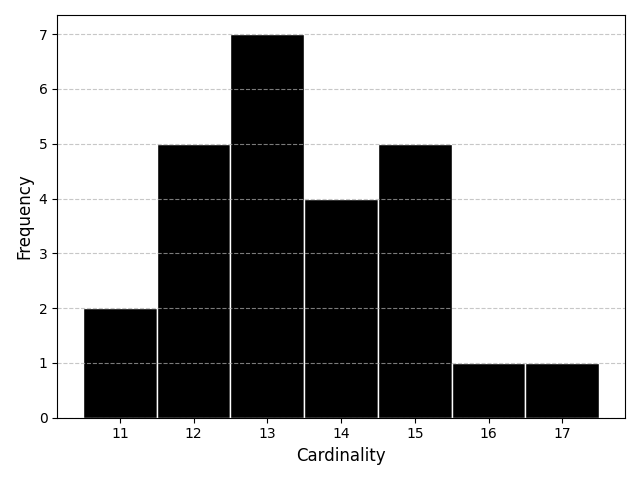
\includegraphics[width=\textwidth]{../figures/wine_cardinalities}
        \caption{Wine Dataset}
        \label{fig:wine_cardinalities}
    \end{subfigure}
    \hfill
    % Subfigure for Iris dataset
    \begin{subfigure}[b]{0.3\textwidth}
        \centering
        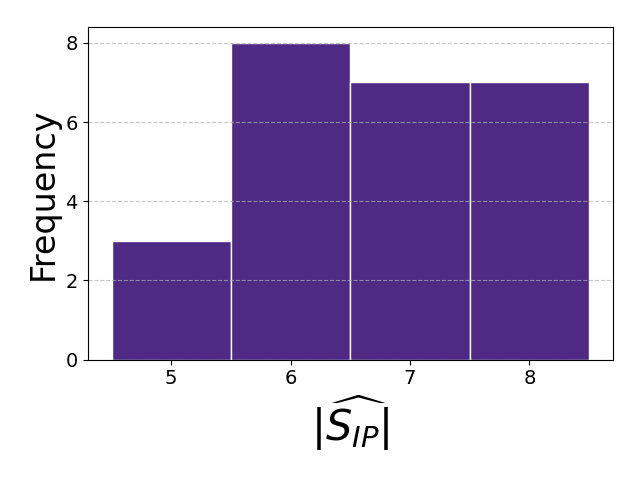
\includegraphics[width=\textwidth]{..//figures/iris_cardinalities}
        \caption{Iris Dataset}
        \label{fig:iris_cardinalities}
    \end{subfigure}
    \hfill
    % Subfigure for Ethanol dataset
    \begin{subfigure}[b]{0.3\textwidth}
        \centering
        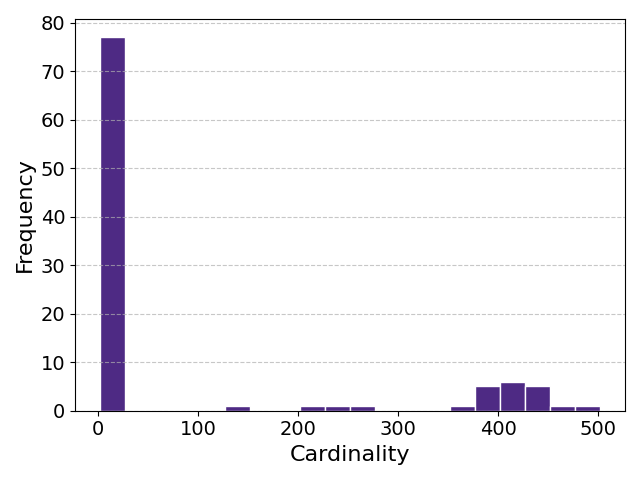
\includegraphics[width=\textwidth]{../figures/ethanol_cardinalities}
        \caption{Ethanol Dataset}
        \label{fig:ethanol_cardinalities}
    \end{subfigure}
    \caption{Support Cardinalities for Wine, Iris, and Ethanol datasets}
    \label{fig:support_cardinalities}
\end{figure}

\newpage

\subsection{Proposition \ref{prop:unitary_selection} deep dive}
\label{sec:deep_dive}

As mentioned in Section \ref{sec:discussion}, the conditions under which the restriction $P=D$ in Proposition \ref{prop:unitary_selection} may be relaxed are of theoretical and practical interest.
The results in Section \ref{sec:experiments} show that there are circumstances in which the \greedy~ performs better than \tsip, so clearly \tsip~ does not always achieve a global optimum.
Figure \ref{fig:comparison_losses} gives results on the line of inquiry about why this is the case based on the reasoning presented in Section \ref{sec:discussion}.
In these results a two-stage algorithm achieves the global optimum of a slightly different brute problem, namely brute optimization of the multitask basis pursuit penalty $\|\cdot \|_{1,2}$.
That is, brute search on $\|\cdot \|_{1,2}$ gives the same result as the two stage algorithm with brute search on $\|\cdot \|_{1,2}$ subsequent to isometry pursuit.
This suggests that failure to select the global optimum by \tsip~ is in fact only due to the mismatch between global optimums of brute optimization of the multitask penalty and the isometry loss given certain data.
Theoretical formalization, as well as investigation of what data configurations this equivalence holds for, is a logical follow-up.

\begin{figure}[t] % Place at the top of the page
    \centering
    % Top-left plot
    \begin{subfigure}[b]{0.45\textwidth}
        \centering
        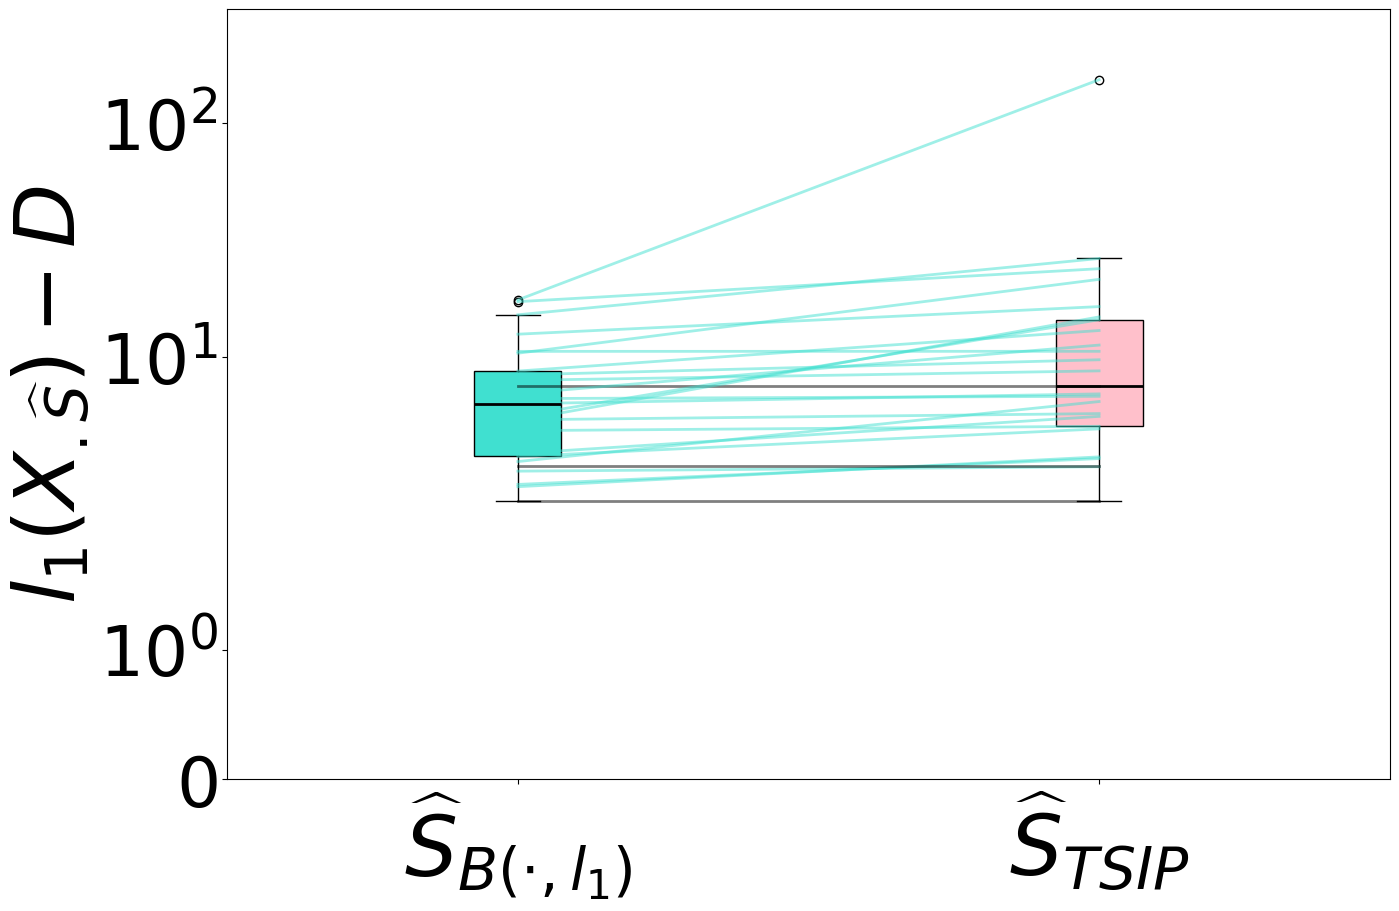
\includegraphics[width=\textwidth]{../figures/iris_standardized_0p1_1p0_isometry_losses}
        \caption{Iris Isometry Losses}
        \label{fig:iris_isometry_losses}
    \end{subfigure}
    \hfill
    % Top-right plot
    \begin{subfigure}[b]{0.45\textwidth}
        \centering
        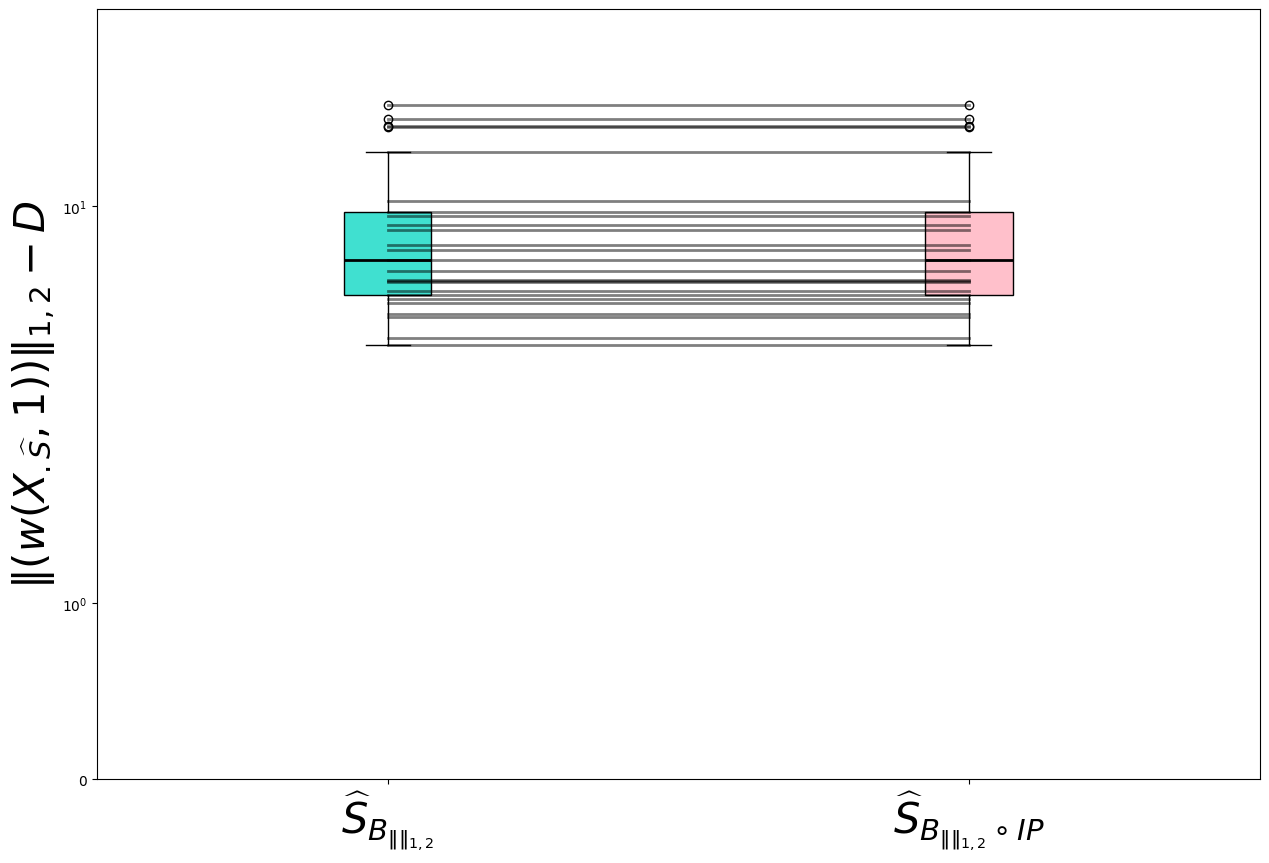
\includegraphics[width=\textwidth]{../figures/iris_standardized_0p1_1p0_group_lasso_losses}
        \caption{Iris Multitask Losses}
        \label{fig:iris_group_lasso_losses}
    \end{subfigure}

    \vspace{0.5cm} % Add vertical spacing between rows

    % Bottom-left plot
    \begin{subfigure}[b]{0.45\textwidth}
        \centering
        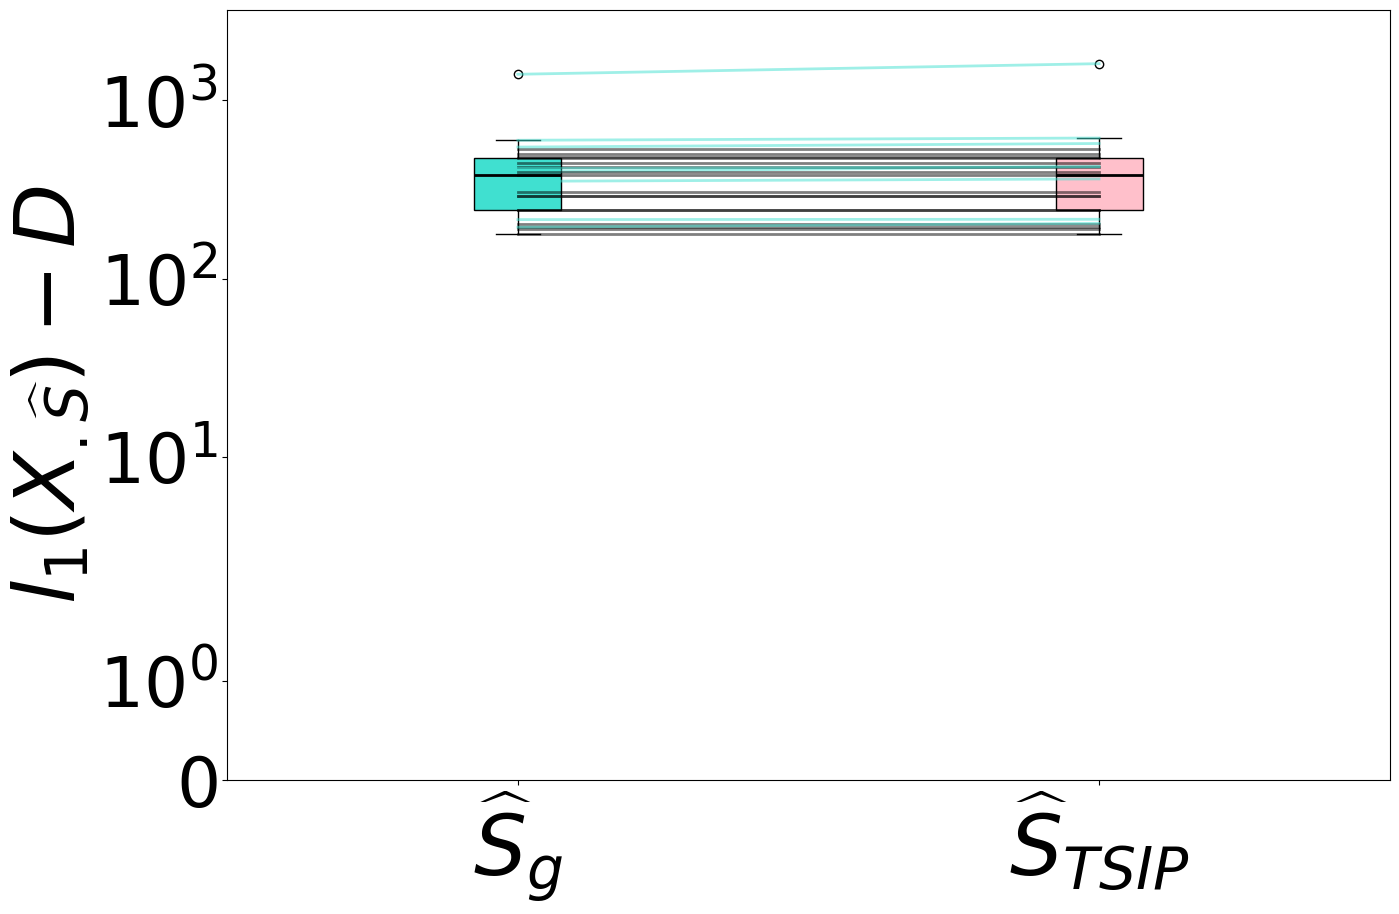
\includegraphics[width=\textwidth]{../figures/wine_standardized_0p1_1p0_isometry_losses}
        \caption{Wine Isometry Losses}
        \label{fig:wine_isometry_losses}
    \end{subfigure}
    \hfill
    % Bottom-right plot
    \begin{subfigure}[b]{0.45\textwidth}
        \centering
        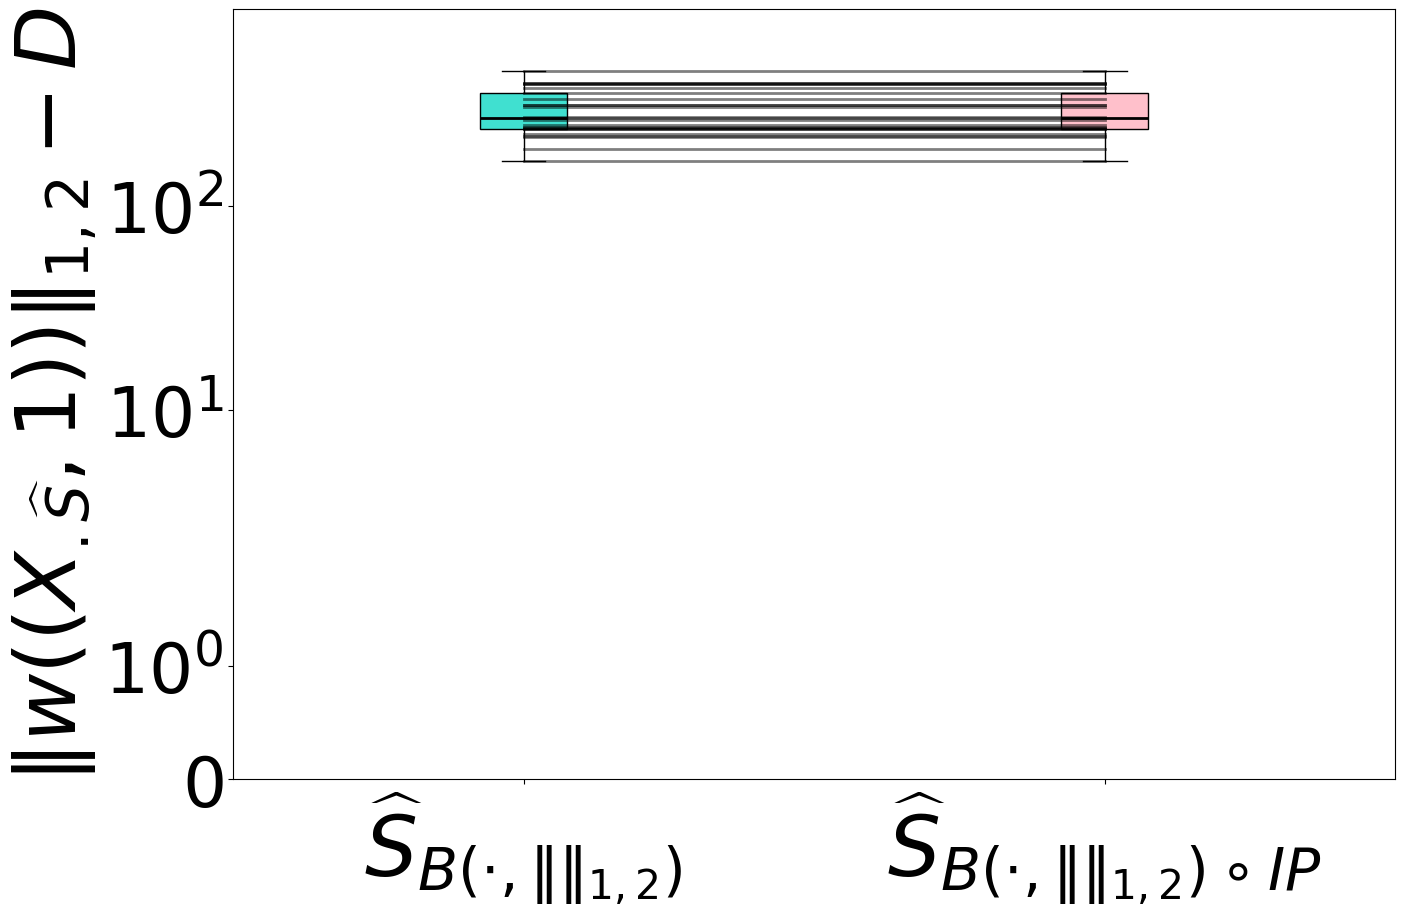
\includegraphics[width=\textwidth]{../figures/wine_standardized_0p1_1p0_group_lasso_losses}
        \caption{Wine Multitask Losses}
        \label{fig:wine_group_lasso_losses}
    \end{subfigure}
    \caption{Comparison of Isometry and Group Lasso Losses across $25$ replicates for randomly downsampled Iris and Wine Datasets with $(P,D) = (4,15)$ and $(13, 18)$, respectively.
    Note that this further downsampling compared with Section \ref{sec:experiments} was necessary to compute global minimizers of \brute.
    Lower brute losses are shown with turquoise, while lower two stage losses are shown with pink.
    Equal losses are shown with black lines.}
    \label{fig:comparison_losses}
\end{figure}

\newpage

\subsection{Timing}
\label{sec:timing}

While wall-time of algorithms is a non-theoretical quantity that depends on implementation details, it provides valuable context for practitioners.
We therefore report the following runtimes on a 2021 Macbook Pro.
The particularly high variance for brute force search in the second step of \tsip~ is likely due to the large cardinalities reported in Figure \ref{fig:support_cardinalities}.

\begin{table}[H]
\centering
\begin{tabular}{|c|c|c|c|}
\toprule
Name & IP & 2nd stage brute & Greedy \\
\midrule
Iris & 1.24 ± 0.02 & 0.00 ± 0.00 & 0.02 ± 0.00 \\
Wine & 2.32 ± 0.17 & 0.13 ± 0.12 & 0.03 ± 0.00 \\
Ethanol & 8.38 ± 0.57 & 0.55 ± 1.08 & 0.07 ± 0.01 \\
\bottomrule
\end{tabular}
\caption{Algorithm runtimes in seconds across replicates.}
\end{table}